\documentclass[]{article}

\usepackage{amsmath}
\usepackage[]{graphicx}
\usepackage{subfigure}
\usepackage[latin1]{inputenc}
\usepackage{comment}
\usepackage{url}
%\usepackage{biblatex} 
%\usepackage[pdftex]{graphicx}
\usepackage{anysize}

\providecommand{\e}[1]{\ensuremath{\times 10^{#1}}}

\marginsize{3cm}{3cm}{2cm}{2.5cm}%l r t b

\title{Gaze Enhanced Speech Recognition for Hands-Free HCI}
%\title{Controlling a smart phone using gaze gestures}
%\title{Gaze gestures as an innovative HCI method for smartphone like devices}
 
\author{Matheus Portela, David Rozado}

\setlength\parindent{0pt} %no indentation in paragraphs
% Document starts
\begin{document}

\maketitle

\section{Abstract}
This is the abstract

\section{Introduction}
In computer science speech recognition refers to the computational translation of spoken words into text.

Using speech to create or edit documents and e-mail offers the potential to be a faster a more natural way to interact
with computers as well as a hands-free modality with obvious positive implications for handicapped users or
scenarios were computer users have their hands engaged in other tasks (for example surgeons in the operating room).

Although there has been a significant increase in the accuracy performance of speech recognition software, error
rates still make the technology cumbersome to use for everyday interaction  and it still requires a relatively long
learning curve to master it.

The correction of errors can be carried out manually with a traditional keyboard and mouse to select and retype the
misrecognized word. This modality can be perfectly valid for some scenarios, but this interaction modalities is not
hands-free anymore.  Correcting misrecognized with voice is an alternative that while remaining hands-free is extremely
error-prone and frustrating for users, especially when trying to correct ``difficult'' words or when being used by users
with an accent.

In this work, we propose the enhancement of speech recognition software with gaze tracking technology to speed up the
correction of misrecognized words and to make speech recognition truly hands-free.

A gaze tracking system tracks the point of regard (PoR) of the user on the screen by monitoring the users pupils while
sitting in front of a computer \cite{Rozado2012a}.

In the experimental part of his work, we compared three modalities of correcting misrecognized words during  a speech
recognition task:
\begin{itemize}
  \item usage of the traditional keyboard and mouse
  \item usage of voice
  \item usage of gaze
\end{itemize}



\section{Methodology}
Methodology introduction

\subsection{Eye Tracking}
Eyes are used by humans to obtain information about the surroundings and to
communicate information. When something attracts our attention, we position our
gaze on it, thus performing a \textit{fixation}. A fixation usually has a
duration of at least 150 milliseconds (ms). The fast eye movements that
occur between fixations are known as \textit{saccades}, and they are used to
reposition the eye so that the object of interest is projected onto the fovea.
The direction of gaze thus reflects the focus of 
\textit{attention} and also provides an indirect hint for \textit{intention}
\cite{velichkovsky}.


A video-based gaze tracking system seeks to find where a person is looking, i.e.
the Point of Regard (PoR), using images obtained from the eye by one
or more cameras. Most systems employ infrared
illumination that is invisible to the human eye and hence it is not distracting
for the user. Infrared light improves image contrast and produces a reflection
on the cornea, known as corneal reflection or glint. Eye features such as the
corneal reflections and the center of the pupil/iris can be used to estimate the
PoR. Figure \ref{screenGazeTracker} shows a screenshot of an eye being tracked
by the open-source ITU Gaze Tracker \cite{lowcostitugazetracker}. In this case,
the center of the pupil and two corneal reflections are the features being
tracked.


\begin{figure}[ht]
\begin{center}
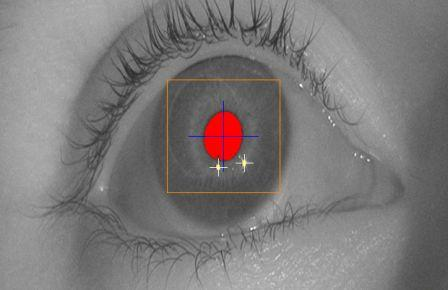
\includegraphics[width=0.5\textwidth, height=30mm]{figures/screenGazeTracker.jpg}
\vspace{-3mm}
\end{center}
\caption{\textbf{The Open Source ITU Gaze Tracker tracking one eye.} The
features tracked in the image are the pupil center and two corneal reflections.}
\label{screenGazeTracker}
\end{figure}


\subsection{Experimental Setup}
The video at \url{http://www.youtube.com/watch?v=xdBoNsMthr8} provides a good overview of the
experimental setup.

\section{Results}
The user study generated the results enumerated next.

The average time  for each correction modality to achieve the target sentence is displayed in Figure \ref{timeFig}.
A Levenes' test for equal variance for the 3 correction modalities failed ($p=2.1$). Hence, the results of the
ANOVA analysis need to be interpreted with caution. The F-test produced a value of $F=17.43$, $p=1.44\e{-06}$.
A Posthoc Bonferroni-Holm test indicated significant differences between the voice-mouse, gaze-mouse and gaze-voice
modalities with $p=4.24\e{-06}$, $p=3.6\e{-05}$ and $p=0.02$, respectively. 
 

\begin{figure}[ht]
\begin{center}
\vspace{-3mm}
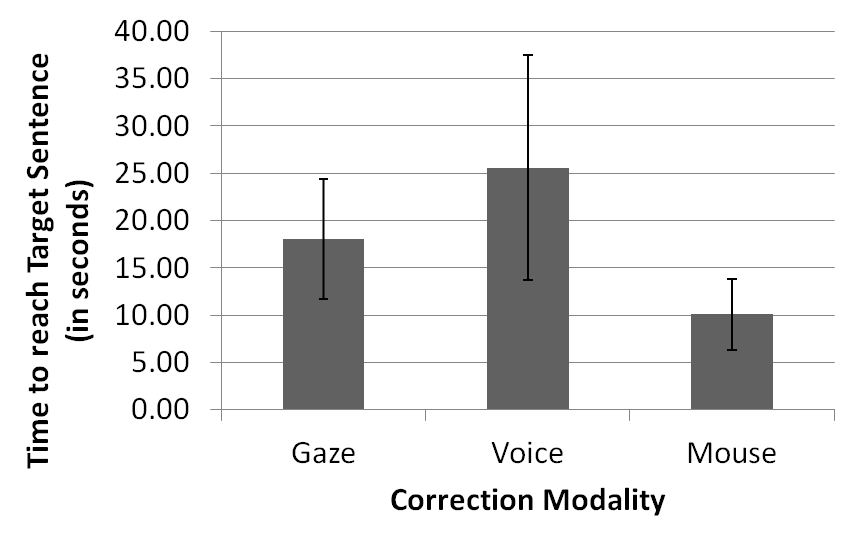
\includegraphics[width=0.95\textwidth,height=50mm]{figures/time.png}
\end{center}
\caption{\textbf{Average Time Required to Achieve Target Sentence.} The figure displays the average time of the
experimental trials required by each correction modality to reach the target sentence.}
\label{timeFig}
\end{figure}


Figure \ref{mouseDisplacement} shows the average displacement of the mouse during each experimental trial for each
correction modality. Again, a Levene's test failed to find equal variance among experimental conditions. The ANOVA
showed significant differences between groups,  $F=19.27$, $p=4.82\e{-07}$. A Posthoc Bonferroni-Holm test found
significant differences between the gaze-mouse and voice-mouse modalities,  $p=4.95\e{-06}$,
$p=3.8\e{-04}$ respectively but now between the gaze-voice modalities.


\begin{figure}[ht]
\begin{center}
\vspace{-3mm}
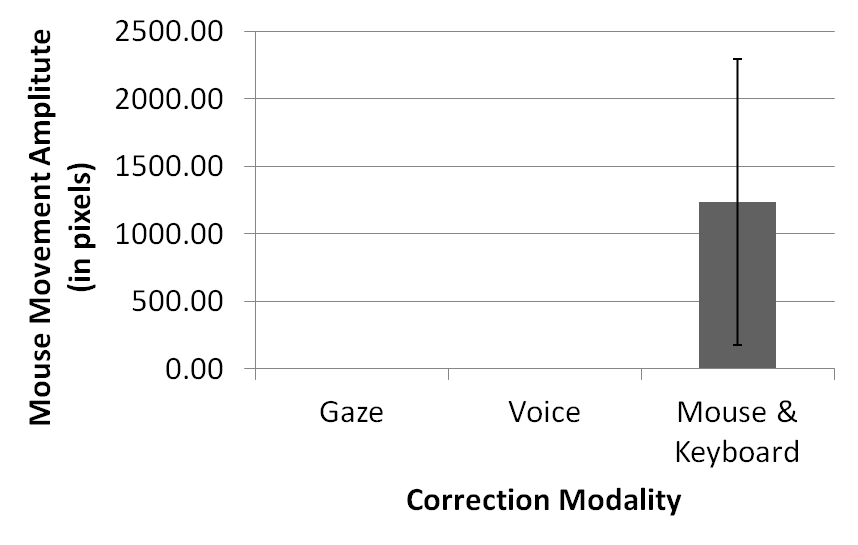
\includegraphics[width=0.95\textwidth,height=50mm]{figures/mouseDisplacement.png}
\end{center}
\caption{\textbf{Average Mouse Movement Amplitude.} The figure displays the average mouse movement amplitude (in pixels)
required by each correction modality to reach the target sentence during the experimental trials.}
\label{mouseDisplacement}
\end{figure}

The average number of keystrokes required from the subjects to achieve the target sentence by each correction modality
during the experimental trials is shown in Figure \ref{keystrokes}. Again a Levene's test failed to assume equal
variance. Nonetheless the ANOVA analysis showed statistically significant differences between the results of the
difference correction modalities, $F=36.79$, $p=8.29\e{-11}$. 

\begin{figure}[ht]
\begin{center}
\vspace{-3mm}
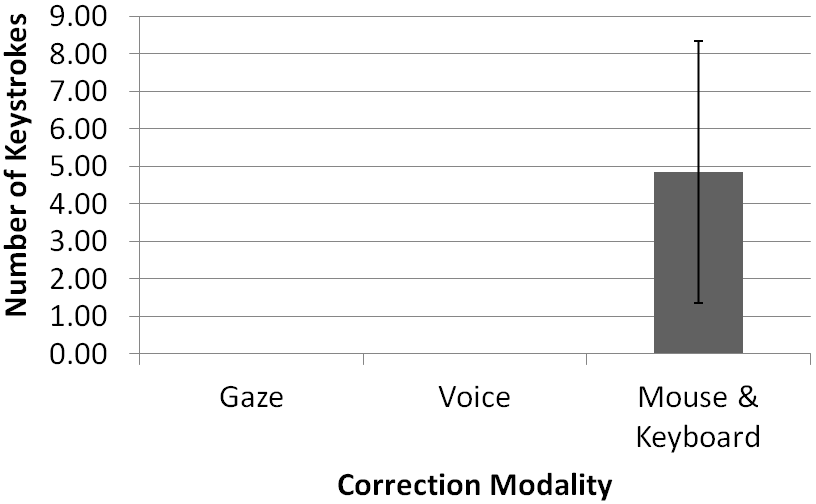
\includegraphics[width=0.95\textwidth,height=50mm]{figures/keystrokes.png}
\end{center}
\caption{\textbf{Number of Keystrokes.} The figure displays the average mouse movement amplitude (in pixels)
required by each correction modality to reach the target sentence during the experimental trials.}
\label{keystrokes}
\end{figure}


Figure \ref{failFig} shows the average number of trials in which the user was unable to reach the target sentence in the
allotted time of 60 seconds using the given correction modality. The Levene's test also failed to determine equal
variance. The ANOVA analysis showed statistically significant differences between the results of the
difference correction modalities, $F=17.92$, $p=1.07\e{-06}$.   A Posthoc Bonferroni-Holm test found
significant differences between the voice-mouse modalities, $p=6.62\e{-06}$, gaze-mouse modalities $p=9.23\e{-05}$
and gaze-voice modalities $p=4.02\e{-03}$.

\begin{figure}[ht]
\begin{center}
\vspace{-3mm}
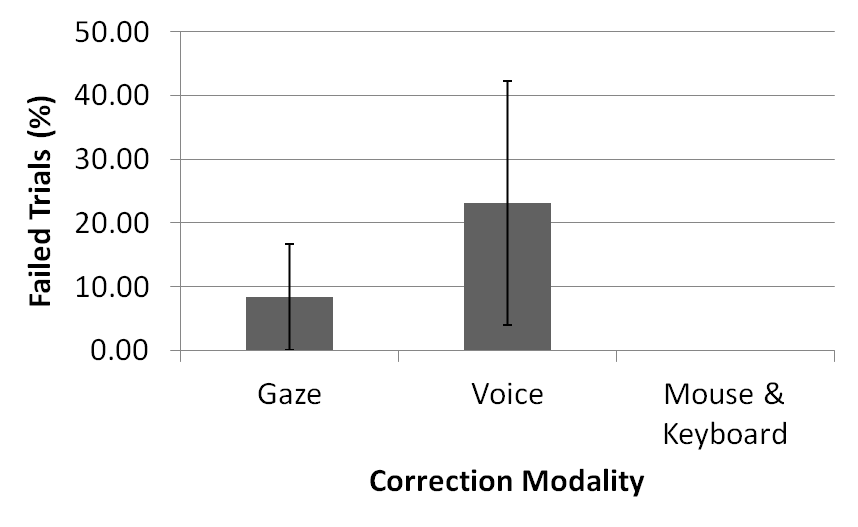
\includegraphics[width=0.95\textwidth,height=50mm]{figures/fail.png}
\end{center}
\caption{\textbf{Number of Failed Trials.} The figure displays the average number of trials in which the user
was unable to reach the given target sentence within the allotted time of 60 seconds.}
\label{failFig}
\end{figure}

The average DL distance between the target sentence and the generated sentence within the 60 seconds time window for
each correction modality is shown in Figure \ref{dldistance}. The ANOVA analysis generated statistically
significant differences between modalities with values $F=11.60$, $p=6.44\e{-05}$. A Posthoc Bonferroni-Holm test found
significant differences between the voice-mouse modalities, $p=5.18\e{-04}$, gaze-voice modalities $p=4.44\e{-03}$
and gaze-mouse modalities $p=1.71\e{-02}$. 

\begin{figure}[ht]
\begin{center}
\vspace{-3mm}
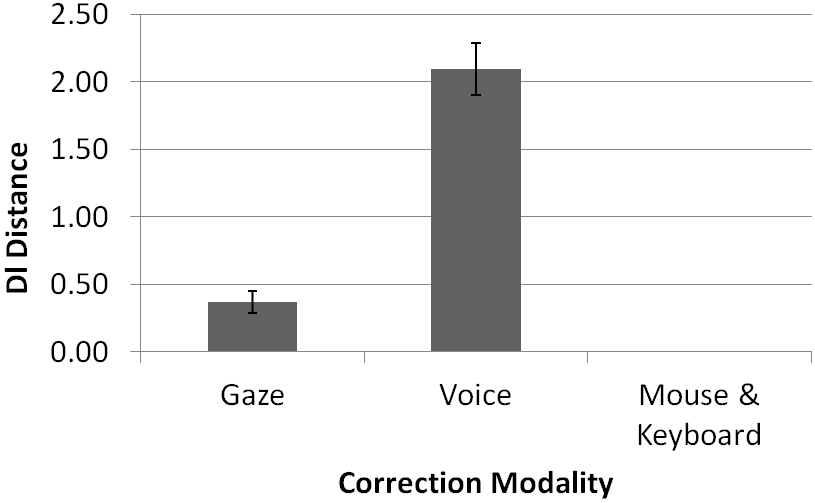
\includegraphics[width=0.95\textwidth,height=50mm]{figures/dldistance.png}
\end{center}
\caption{\textbf{DL Distance.} This figure shows the average DL distance between the target sentence and the generated
sentence.}
\label{dldistance}
\end{figure}


\section{Discussion}
Bla bla


\bibliographystyle{plain}
\bibliography{library}

\end{document}
